% How the research was carried out (action strategy)

\chapter{Methodology} \label{chap:ch3}

\section{NegotiationArena Framework}
\subsection{Games}
\subsection{Evaluation Metrics}

\section{Models and Infrastructure}

\begin{table}[htbp]
\centering
\small
\caption{Open-weight models used across all experiments. Gemma, Qwen, and
Mistral-Small are loaded with 8-bit quantization (bitsandbytes); the Ministral
models are released already quantized to FP8 and are used at that
native precision. VLM models are loaded with a vision-language (image-text-to-text) head; Qwen
models run with thinking mode disabled.}
\label{tab:experiment-models}
\begin{tabular}{lllll}
\toprule
\textbf{Tier} & \textbf{Model} & \textbf{Params} & \textbf{Quantization} & \textbf{Notes} \\
\midrule
\multirow{3}{*}{Very small}
  & Gemma 3 4B IT            & 4B  & 8-bit (bnb)    & --- \\
  & Ministral 3 8B Instruct  & 8B  & FP8 (native)   & VLM \\
  & Qwen3.5 9B               & 9B  & 8-bit (bnb)    & Thinking off \\
\midrule
\multirow{3}{*}{Small}
  & Gemma 3 12B IT           & 12B & 8-bit (bnb)    & --- \\
  & Ministral 3 14B Instruct & 14B & FP8 (native)   & VLM \\
  & Qwen3 14B                & 14B & 8-bit (bnb)    & Thinking off \\
\midrule
\multirow{3}{*}{Medium}
  & Gemma 3 27B IT           & 27B & 8-bit (bnb)    & --- \\
  & Mistral-Small 3.2 24B    & 24B & 8-bit (bnb)    & VLM \\
  & Qwen3.5 27B              & 27B & 8-bit (bnb)    & Thinking off \\
\bottomrule
\end{tabular}
\end{table}

\section{Benchmarking Open-Weight LLMs}

\section{Self-Refine}

\begin{figure}
    \centering
    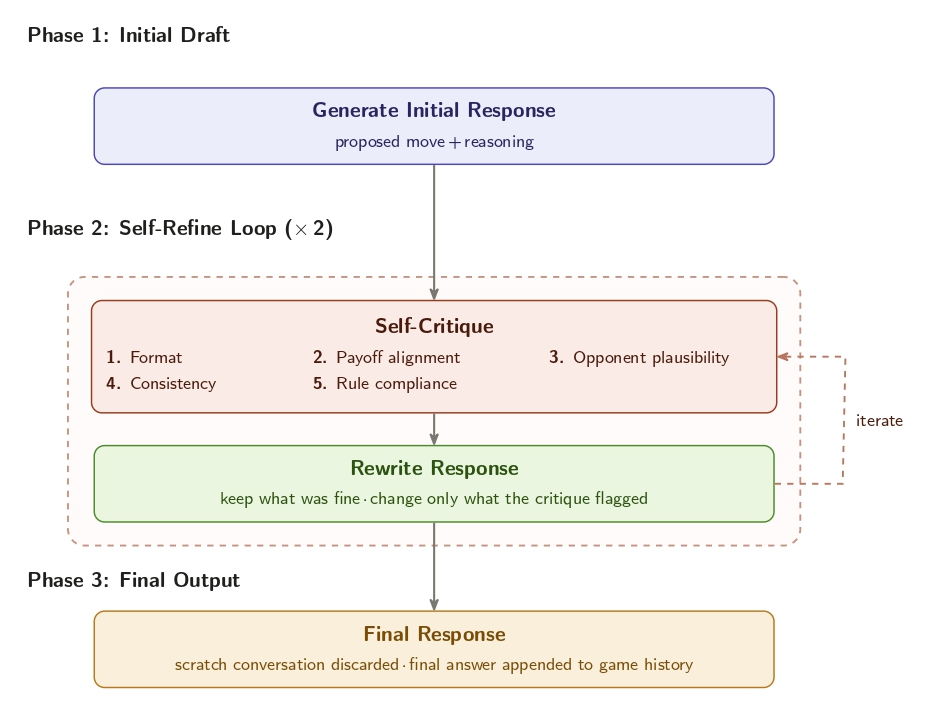
\includegraphics[width=0.9\linewidth]{figures//methodology/SelfRefine___Figure.jpg}
    \caption{Self-Refine process. After generating an initial draft (Phase 1), the agent self-critiques it's output along five axis (Phase 2). Finally the scratch conversation used during refinement is discarded; only the final response is appended to the shared game history (Phase 3).}
    \label{fig:self_refine_loop}
\end{figure}

\section{Team Negotiation}

\begin{figure}
    \centering
    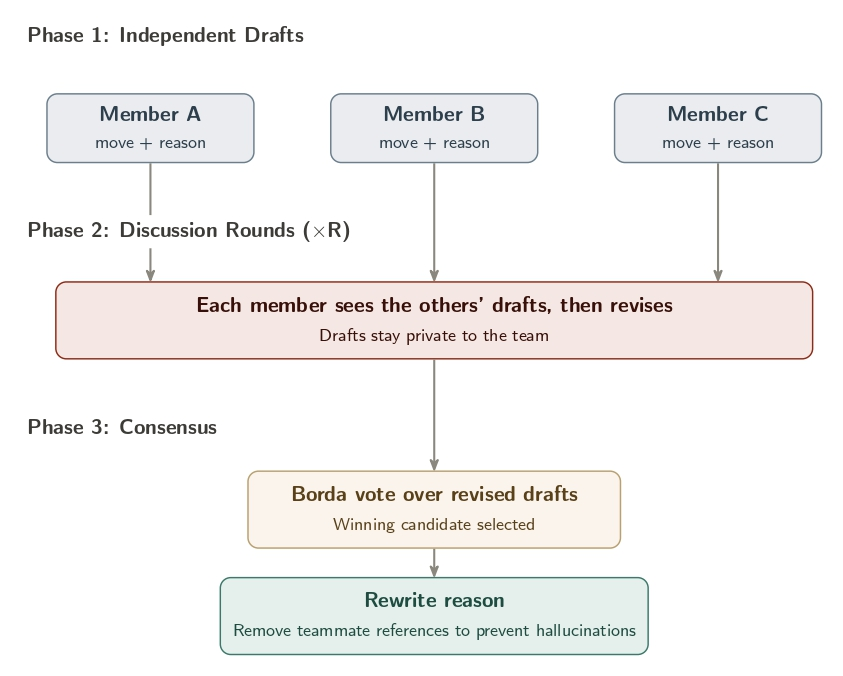
\includegraphics[width=0.9\linewidth]{figures/methodology/team_based_negotiation_fig.png}
    \caption{Team deliberation process. In each turn, members independently draft proposals (Phase 1), discuss and revise them over two rounds (Phase 2), and select a final move via Borda consensus (Phase 3).}
    \label{fig:placeholder}
\end{figure}
